\pagebreak
\pagenumbering{arabic}
\chapter{Introduction}


\section{The mechanisms of Functional Magnetic Resonance Imaging}

\subsection{Blood Oxygen Level Dependent Signal \textit{(BOLD)}}

% Short abstract of subsection.
The \gls{BOLD} signal , captured in \gls{fMRI} detects changes in \gls{HbR} driven by localized changes in brain blood flow and blood oxygenation, which are coupled to underlying neuronal activity by a process termed neurovascular coupling. \gls{fMRI} relies upon the measurement of T2* relaxation, which is sensitive primarily to local concentrations of πaramagnetic \gls{HbR} in venous blood, rendering the latter a naturally occurring contrast agent. Interpretation of the \gls{fMRI} \gls{BOLD} signal is intrinsically linked to understanding the underlying physiological and metabolic processes in the brain that modulate blood flow.

\begin{wrapfigure}{l}{0.4\textwidth}
   \centering
   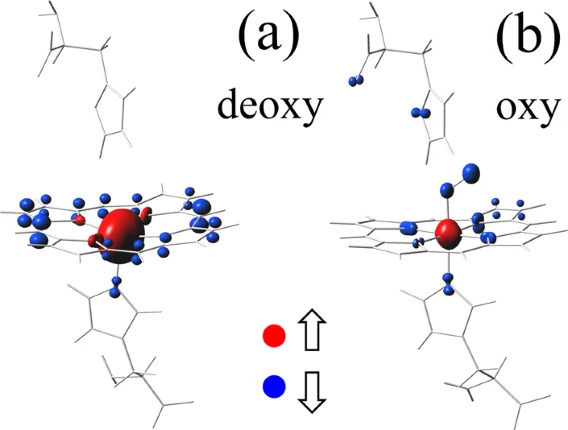
\includegraphics[width = 0.4\textwidth, height = 4.5cm]{assets/images/DeoxyHb_magnetic.jpg}
   \caption{Illustation of magnetic-moment density \textbf{M(r)} for the \textbf{(a)} \gls{HbR} and \textbf{(b)} \gls{HbO} heme clusters at \textit{T = 150K}. The magnitude of \textbf{M(r)} at an atomic site is proportional to the volume of the bubble at that site \cite{Mayda2020} Fig. 2 p.2).}
   \label{fig:HbMagnetic}
\end{wrapfigure}

% How BOLD manifests.
The \gls{BOLD} effect related to neural activity arises because of two distinct phenomena. The first is that when \gls{Hb}-the molecule in blood that carries oxygen-lose the oxygen to become \gls{HbR}, its magnetic properties change in a subtle way: \gls{HbR} is paramagnetic, and alters the magnetic susceptibility of blood, whereas \gls{HbO} and the surrounding tissue \ce{H2O} are diamagnetic \autoref{fig:HbMagnetic}. The difference in susceptibility between blood vessels and the surrounding tissue creates local magnetic field distortions that decrease the net \gls{MR} signal. In the brain, a typical \gls{OEF}-the fraction of \ce{O2} carried by an element of blood that is removed in passing through the capillary bed-is approximately 40\% and in a 3 T magnetic field this level of \gls{HbR} in the veins and capillaries is sufficient to reduce the \gls{MR} signal by about 10\% in the baseline state, compared to what it would be if no \gls{HbR} was present. 

The combination of the aforementioned with the biophysical phenomenon, that when a brain area is activated, the blood flow increases-via a process called the haemodynamic response-to a greater degree than the oxygen metabolic rate, produces a useful basis for an experimental signal aqcuisition technique. The second phenomenon leads to a reduction in the \gls{OEF}, a seemingly paradoxical scenario in which the venous blood is more oxygenated, despite the increase in oxygen metabolic rate, because the blood flow has increased to a greater extent. Taken together, these two phenomena produce the \gls{BOLD} effect, a local increase in the \gls{MR} signal due to a reduction in the \gls{OEF} during increased neural activity. \cite{Buxton2013}

% Misconception tackled.
A prevailing misconception is that \gls{BOLD} provides a direct measurement of neuronal oxygen consumption. However, this is generally not the case; classic positive \gls{BOLD} signals, seen in response to functional stimuli, represent a decrease in \gls{HbR} and thus an overoxygenation of the responding region \cite{Attwell2002}. These positive \gls{BOLD} responses correspond to a local, actively actuated, increase in blood flow and volume, which brings blood in sufficient excess to increase local oxygenation levels \cite{Raichle1998}. This response typically begins within about 500ms and peaks 3-5 seconds after stimulus onset \autoref{fig:BOLD}, even for short stimuli lasting less than 1 second, with more complex dynamics for prolonged stimuli.

\begin{figure}[H]
    \centering
    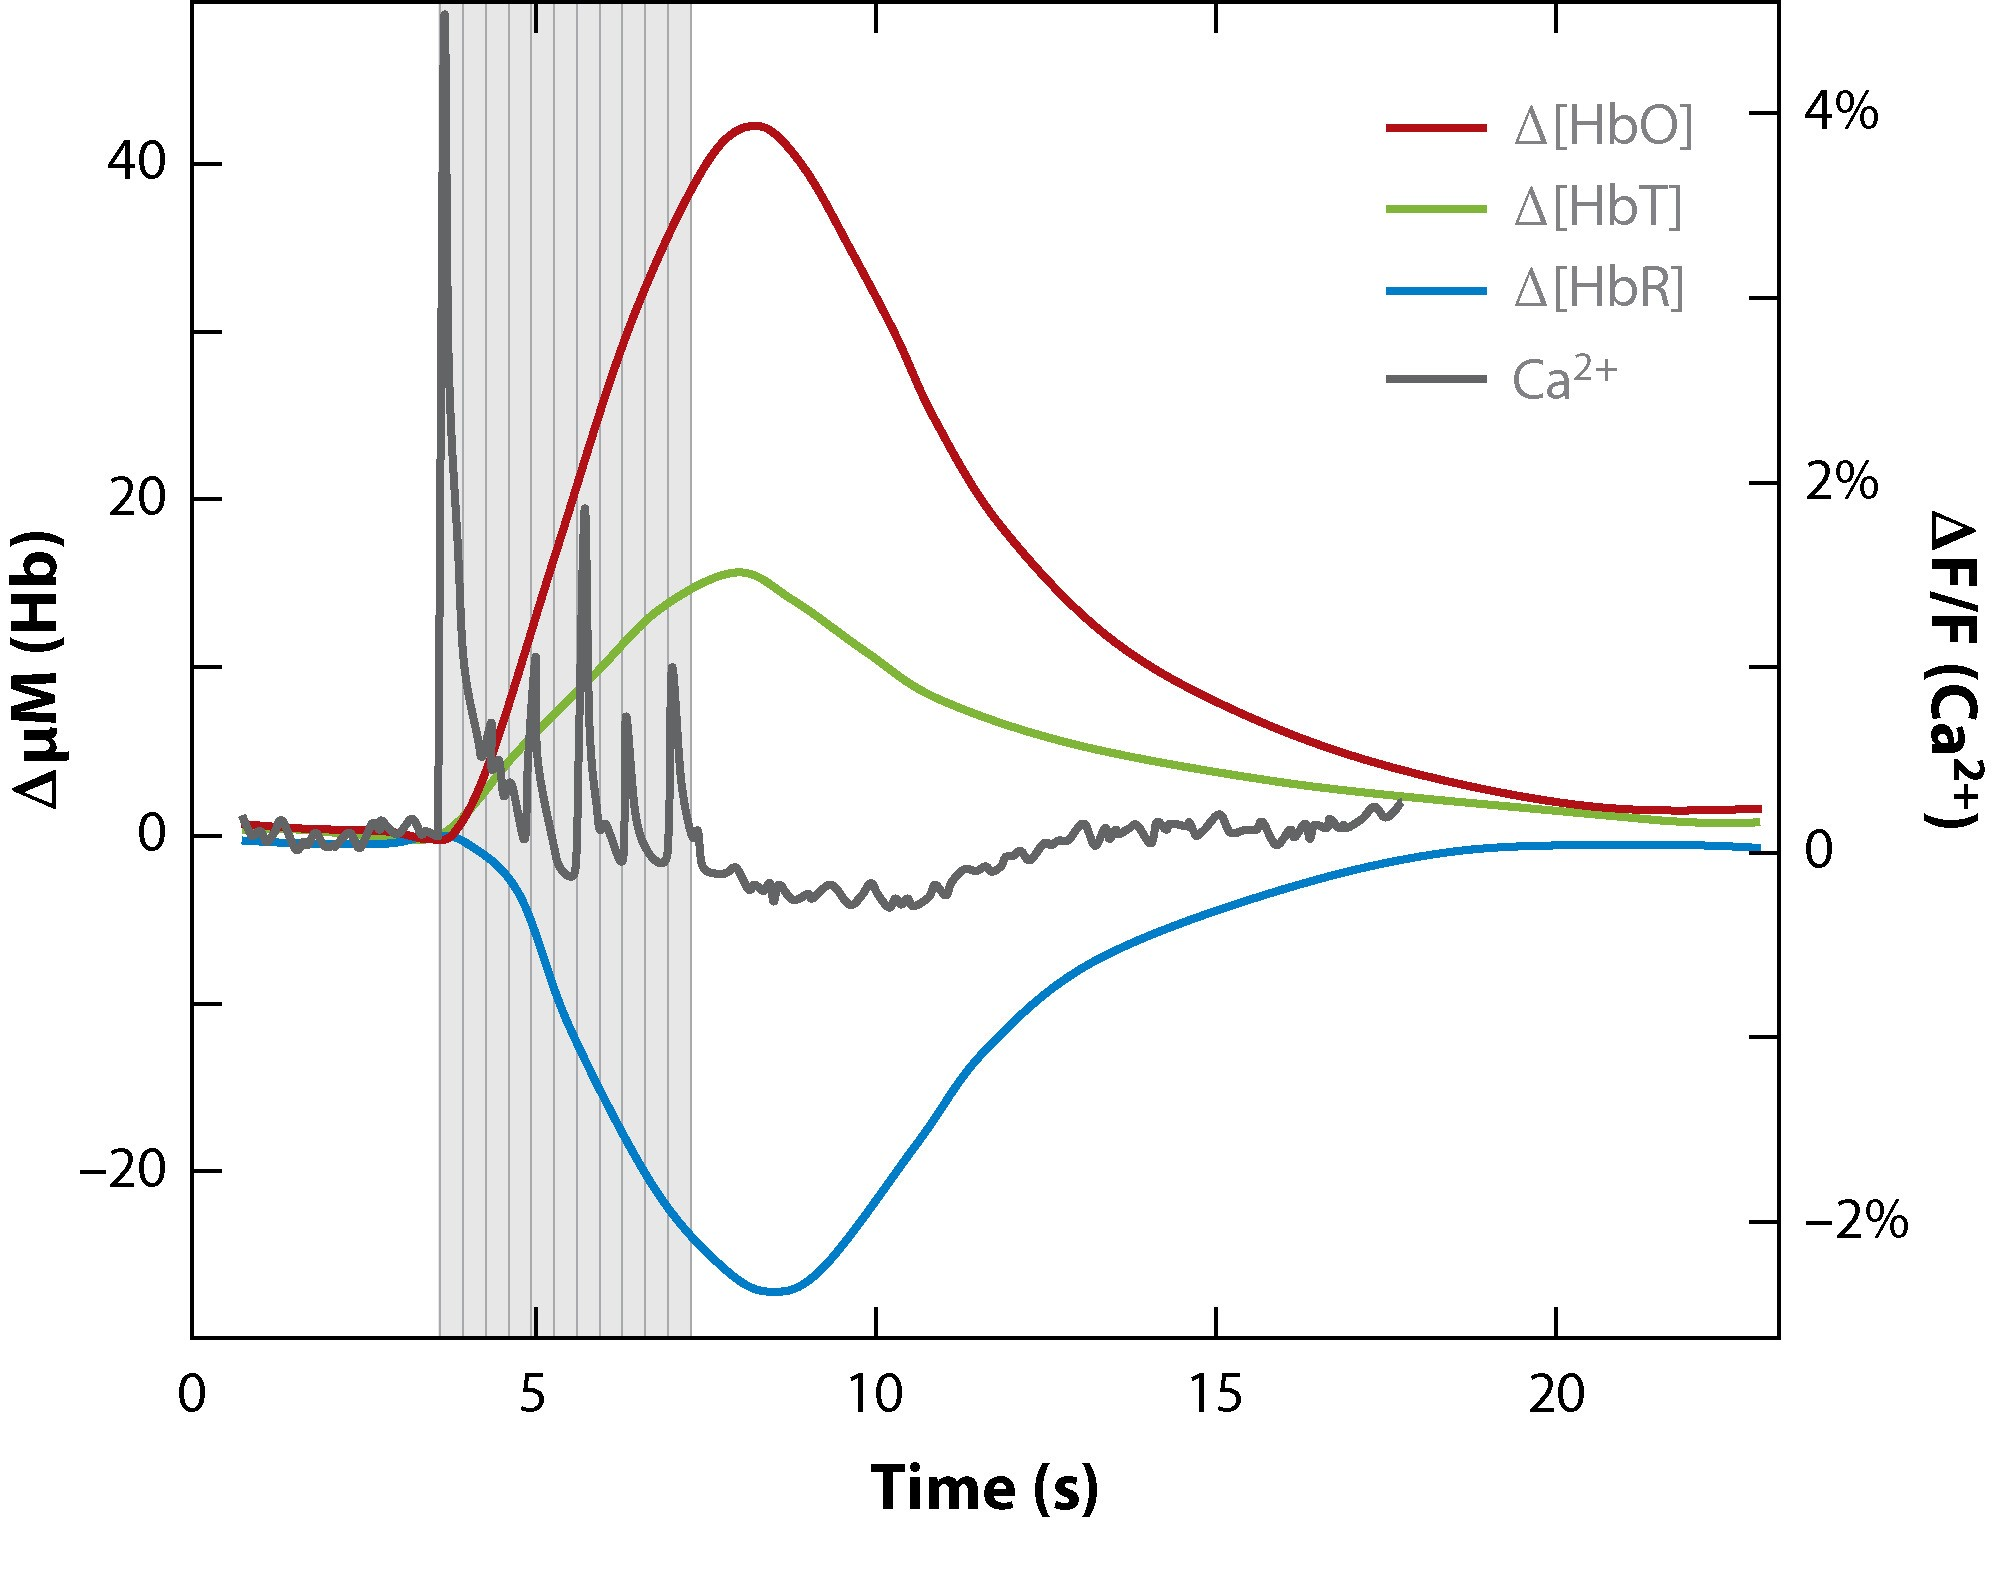
\includegraphics[width = 0.75\textwidth]{assets/images/Hb_flactuations_BOLD.jpg}
    \caption{Stimulus-evoked response in somatosensory cortex of rats. Noteably, there is a distinct increase in \gls{HbT} corresponding to vessel dilation and an increase in the number of red blood cells per unit volume of cortex, consistent with an increase in blood flow. \gls{HbO} increases while \gls{HbR} decreases, indicating a net overoxygenation of the region. The \gls{fMRI} \gls{BOLD} is sensitive to changes in \gls{HbR}, where stimulus-evoked "positive \gls{BOLD}" corresponds to the decrease in \gls{HbR} shown here \cite{Hillman2007} Fig. 2 p.4).}
    \label{fig:BOLD}
\end{figure}

% Broad finishing statements.
A range of cellular mechanisms, including astrocytes, pericytes, and interneurons, have been proposed to play a role in neurovascular coupling.\cite{Hillman2014}. For classical interpretation of \gls{BOLD} signals, it is assumed that neurovascular coupling is so robust that any increase in neuronal activity generates a proportional increase in local blood flow, irrespective of brain region, brain development, and pathological state \cite{Logothetis2010}.

\subsection{The HCP WM task experiment}

% Where the data was extracted from.
The data manipulated in this project has been obtained from the \gls{HCP} database, whose overarching purpose is to acquire and share data about the structural and functional connectivity of the human brain. One of the major categories of data in the \gls{HCP} refers to \gls{tfMRI} which assesses seven domains that sample the diversity of neural systems of interest, to a wide range of individuals in the field: 1) visual, motion, somatosensory, and motor systems; 2) category specific representations; 3) working memory or cognitive control systems; 4) language processing (semantic and phonological processing); 5) social cognition (Theory of Mind); 6) relational processing; and 7) emotion processing. \textbf{cite Barch2013, cite HCP somehow?}

\vspace{3cm}

\begin{wrapfigure}{r}{0.4\textwidth}
    \centering
    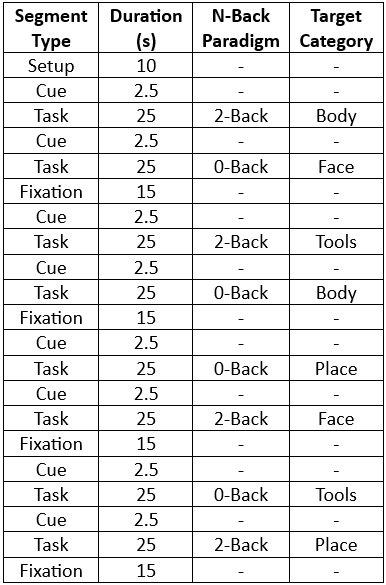
\includegraphics[width = 0.4\textwidth]{assets/images/WM_mat.png}
    \caption{Display of the exact sequece of events during the \gls{WM} task paradigm.}
    \label{fig:WM_mat}
\end{wrapfigure}

% How the experiment was conducted.
The domain which is presently being examined is that of \gls{WM} tasks which is combined with category specific representation tasks into the following, single task paradigm. Stimuli were projected onto a computer screen behind the subject's head within the imaging chamber. The screen was viewed by a mirror positioned approximately 8 cm above the subject's face. Participants were presented with blocks of trials that consisted of pictures of places, tools, faces and body parts (non-mutilated parts of bodies with no "nudity"). Within each run, the four different stimulus types were presented in seperate blocks. Also, within each run, half of the blocks use a 2-back \gls{WM} task and half use a 0-back \gls{WM} task (as a working memory comparison). A 2.5 second cue indicated the task type (and target for 0-back) at the start of the block. Each of the two runs contains eight task blocks (10 trials of 2.5 seconds each, for 25 seconds) and four fixation blocks (15 seconds). On each trial, the stimulis is presented for 2 seconds, followed by a 500ms \gls{ITI}. The procedure is showcased in order in \autoref{fig:WM_mat}.














%\subsection{T1 and T2,T2* times in fMRI?}
